\begin{figure}[p]\centering
\caption[Refusal-signal separability by language]{Refusal-signal separability at index 22. Blue circles use each model\textquotesingle s pooled direction on its estimation rows. Orange diamonds average the six directions learned in other languages and evaluated on the indicated target language. The dashed line is chance ranking ($0.5$). The summaries use different direction-estimation procedures; their gap is descriptive, not a held-out performance loss. All transfer pairs share some question identities.}

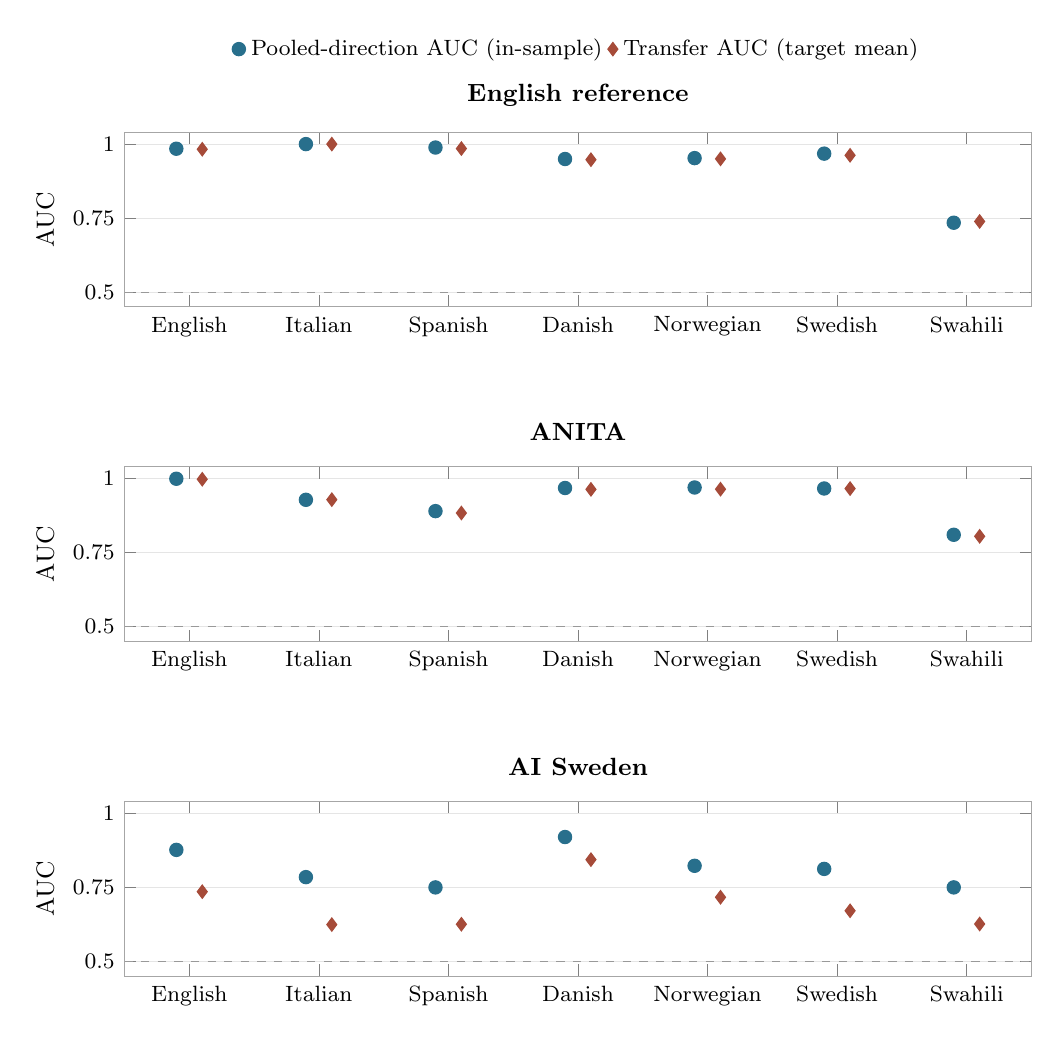
\begin{tikzpicture}
\definecolor{mechblue}{HTML}{286F8C}\definecolor{mechorange}{HTML}{A64B39}
\begin{axis}[width=13.1cm,height=3.8cm,at={(0,-0.0cm)},anchor=north west,xmin=-.5,xmax=6.5,ymin=.45,ymax=1.04,ytick={.5,.75,1},ylabel={AUC},xtick={0,1,2,3,4,5,6},xticklabels={English,Italian,Spanish,Danish,Norwegian,Swedish,Swahili},tick label style={font=\footnotesize},label style={font=\small},title={English reference},title style={font=\small\bfseries},axis line style={black!35},ymajorgrids,grid style={black!10},legend style={font=\footnotesize,draw=none,at={(.5,1.35)},anchor=south,legend columns=2}]
\addplot[black!40,dashed,forget plot] coordinates {(-.5,.5)(6.5,.5)};
\addplot[only marks,mark=*,mark size=2.4pt,color=mechblue] coordinates {(-0.1,0.984375000000) (0.9,1.000000000000) (1.9,0.988425925926) (2.9,0.949652777778) (3.9,0.952651515152) (4.9,0.967803030303) (5.9,0.734375000000)};
\addplot[only marks,mark=diamond*,mark size=2.4pt,color=mechorange] coordinates {(0.1,0.982638888889) (1.1,1.000000000000) (2.1,0.984953703704) (3.1,0.947337962963) (4.1,0.950126262626) (5.1,0.962121212121) (6.1,0.738715277778)};
\legend{Pooled-direction AUC (in-sample),Transfer AUC (target mean)}
\end{axis}
\begin{axis}[width=13.1cm,height=3.8cm,at={(0,-4.25cm)},anchor=north west,xmin=-.5,xmax=6.5,ymin=.45,ymax=1.04,ytick={.5,.75,1},ylabel={AUC},xtick={0,1,2,3,4,5,6},xticklabels={English,Italian,Spanish,Danish,Norwegian,Swedish,Swahili},tick label style={font=\footnotesize},label style={font=\small},title={ANITA},title style={font=\small\bfseries},axis line style={black!35},ymajorgrids,grid style={black!10},legend style={font=\footnotesize,draw=none,at={(.5,1.35)},anchor=south,legend columns=2}]
\addplot[black!40,dashed,forget plot] coordinates {(-.5,.5)(6.5,.5)};
\addplot[only marks,mark=*,mark size=2.4pt,color=mechblue] coordinates {(-0.1,1.000000000000) (0.9,0.928819444444) (1.9,0.890625000000) (2.9,0.968750000000) (3.9,0.970486111111) (4.9,0.967105263158) (5.9,0.810763888889)};
\addplot[only marks,mark=diamond*,mark size=2.4pt,color=mechorange] coordinates {(0.1,0.998263888889) (1.1,0.929398148148) (2.1,0.884259259259) (3.1,0.964120370370) (4.1,0.964699074074) (5.1,0.966739766082) (6.1,0.805555555556)};
\end{axis}
\begin{axis}[width=13.1cm,height=3.8cm,at={(0,-8.5cm)},anchor=north west,xmin=-.5,xmax=6.5,ymin=.45,ymax=1.04,ytick={.5,.75,1},ylabel={AUC},xtick={0,1,2,3,4,5,6},xticklabels={English,Italian,Spanish,Danish,Norwegian,Swedish,Swahili},tick label style={font=\footnotesize},label style={font=\small},title={AI Sweden},title style={font=\small\bfseries},axis line style={black!35},ymajorgrids,grid style={black!10},legend style={font=\footnotesize,draw=none,at={(.5,1.35)},anchor=south,legend columns=2}]
\addplot[black!40,dashed,forget plot] coordinates {(-.5,.5)(6.5,.5)};
\addplot[only marks,mark=*,mark size=2.4pt,color=mechblue] coordinates {(-0.1,0.876736111111) (0.9,0.784722222222) (1.9,0.750000000000) (2.9,0.920138888889) (3.9,0.822916666667) (4.9,0.812500000000) (5.9,0.750000000000)};
\addplot[only marks,mark=diamond*,mark size=2.4pt,color=mechorange] coordinates {(0.1,0.735532407407) (1.1,0.624421296296) (2.1,0.625578703704) (3.1,0.843750000000) (4.1,0.716724537037) (5.1,0.671006944444) (6.1,0.626446759259)};
\end{axis}
\end{tikzpicture}
\label{fig:mechanistic-separability-overview}
\fonte{Prepared by the author (2026).}
\end{figure}
